% Template for PLoS
% Version 1.0 January 2009
%
% To compile to pdf, run:
% latex plos.template
% bibtex plos.template
% latex plos.template
% latex plos.template
% dvipdf plos.template

\documentclass[10pt]{article}

% amsmath package, useful for mathematical formulas
\usepackage{amsmath}
% amssymb package, useful for mathematical symbols
\usepackage{amssymb}

% graphicx package, useful for including eps and pdf graphics
% include graphics with the command \includegraphics
\usepackage{graphicx}

% cite package, to clean up citations in the main text. Do not remove.
\usepackage{cite}

\usepackage{color} 

% Use doublespacing - comment out for single spacing
%\usepackage{setspace} 
%\doublespacing


% Text layout
\topmargin 0.0cm
\oddsidemargin 0.5cm
\evensidemargin 0.5cm
\textwidth 16cm 
\textheight 21cm

% Bold the 'Figure #' in the caption and separate it with a period
% Captions will be left justified
\usepackage[labelfont=bf,labelsep=period,justification=raggedright]{caption}

% Use the PLoS provided bibtex style
\bibliographystyle{plos2009}

% Remove brackets from numbering in List of References
\makeatletter
\renewcommand{\@biblabel}[1]{\quad#1.}
\makeatother


% Leave date blank
\date{}

\pagestyle{myheadings}
%% ** EDIT HERE **


%% ** EDIT HERE **
%% PLEASE INCLUDE ALL MACROS BELOW

%% END MACROS SECTION

\begin{document}

% Title must be 150 characters or less
\begin{flushleft}
{\Large
\textbf{Transcriptome variation in response to Marek's disease virus early infection}
}
% Insert Author names, affiliations and corresponding author email.
\\
Likit Preeyanon$^{1}$
C. Titus Brown$^{1,2}$
Hans H. Cheng$^{3,\ast}$
\\
\bf{1} Microbiology and Molecular Genetics, Michigan State University, East Lansing, MI, USA
\\
\bf{2} Computer Science and Engineering, Michigan State University, East Lansing, MI, USA
\\
\bf{3} USDA, ARS, Avian Disease and Oncology Laboratory, East Lansing, MI, USA
\\
$\ast$ E-mail: Corresponding hans.cheng@ars.usda.gov
\end{flushleft}

% Please keep the abstract between 250 and 300 words
\section*{Abstract}
Marek's disease (MD) is caused by highly oncogenic Marek's disease virus (MDV).
Understanding the genetic basis for non-MHC resistance would be of both
fundamental and applied importance.  In this study, using computational
approaches of RNA-Seq data, we identified differentially expressed genes and
isoforms in response to MDV infection from highly inbred chickens lines that are
MD resistant and susceptible, and performed pathway and functional analysis.
Results show that expression of genes and isoforms involved in cell cytoskeleton
and adhesion molecules in line 6 may contribute to resistance of the disease by
limiting T cell activation, which in turn prevents the spread of MDV to
activated T cells.  In addition, we identified exonic single nucleotide
polymorphisms (SNPs) between lines 6 and 7 predicted their role in regulation of
alternative splicing.  Based on our results, we speculate that alternative
splice forms of cell adhesion molecules and cytoskeleton play and important role
in controlling T cell activation in line 6.

% Please keep the Author Summary between 150 and 200 words
% Use first person. PLoS ONE authors please skip this step. 
% Author Summary not valid for PLoS ONE submissions.   
\section*{Author Summary}

\section*{Introduction}

Marek's disease (MD) is an economically significant chicken disease that affects
the poultry industry worldwide with estimated annual loss of \$2 billion loss
has been reported from outbreaks~\cite{morrow2004marek}.  The disease is caused
by the highly oncogenic Marek's disease virus (MDV), an alphaherpesvirus that
induces T-cell lymphomas in susceptible birds.  Vaccination is the primary
control measure, which is effective in reducing incidence of tumor formation.
However, since MD vaccines are not sterilizing, they do not prevent infection or
horizontal spread of the virus.  As a consequence, MDV field strains that
overcome vaccinal protection have arisen repeatedly over time.  Therefore, there
is a need for sustainable alternative controls measures, such as improving
genetic resistance.

Many studies have reported strong associations between MHC alleles and
resistance or susceptibility to MD.  For example, chickens with MHC allele
B\textsuperscript{21} are highly resistant in contrast to chickens with
B\textsuperscript{19} allele which are highly susceptible.  ADOL lines 6 and 7,
both share (B\textsuperscript{2}) allele, yet exhibit different phenotypic
responses to MD; e.g., challenge with JM/102W strain with result in 0 and 100\%
MD incidence for lines 6 and 7, respectively.  Thus, the major unanswered
questions are what genetic factors, especially those that are non-MHC,
contribute to susceptibility and resistance of the disease and what is the main
contributing mechanism.

In the past decades, significant efforts have been spent to study variations in
a global gene expression between resistant and susceptible birds using
microarray and RNA-Seq methods in order to identify non-MHC genes that
contribute to resistance to
MD~\cite{sarson2008transcriptional,morgan2001induction,vallejo1998genetic,yonash1999high,bumstead1998genomic}.
However, none of the studies have investigated differential expression of
alternative isoforms, which are known to play a significant role in many
biological events including immune responses.  In addition, studies have shown
that isoform expression levels can provide better signatures for some
diseases~\cite{zhang2013isoform}.  Changes of isoform expression levels are
governed partly by two types of {\em cis-}regulatory elements: Exon Splicing
Enhancer (ESE) and Exon Splicing Silencer (ESS), which are located within an
exon sequence.  A number of sequence motifs of ESE and ESS have been identified
in human and some other organisms and could be predicted {\em in silico}.
Mutations that disrupt or create those motifs could alter splicing patterns
leading to aberrant alternative splicing.  A number of disease-associated
single-nucleotide polymorphsims in coding regions (SNPs) that affect ESEs and
ESSs have been well characterized~\cite{blencowe2000exonic, wang2007splicing}.
%In fact, 15\% of mutations that cause genetic diseases affect pre-mRNA splicing
%via this mechanism.
Therefore, variations in isoform expression could lead to identification of SNPs
that underlie genetic resistance to MD.  In this article, we reported
differential-expressed genes and isoforms that may contribute to resistance to
MD as well as SNPs that can potentially affect isoform expression levels.

% Results and Discussion can be combined.
\section*{Results and Discussion}

\subsection*{Differential expression results from our method are comparable to
previous studies}

To extensively study gene and isoform expression, we incorporated ENSEMBL gene
models release 73 with {\em de novo} and a reference-guided transcriptome
assembly to build custom gene models.  The models, therefore, include both
ENSEMBL annotated transcripts and putative genes and isoforms.  The advantage of
using custom gene models is it allows an investigation of unannotated genes and
isoforms, which is necessary for in-depth study of an immune system.

Some DE genes have been reported from previous microarray studies were also
found to be differentially expressed in this study.  For example, B6.1 (Bu-1)
gene is known to be down-regulated approximately 2.27 fold in susceptible
chicken with the MHC allele B\textsuperscript{19} at 4
d.p.i~\cite{sarson2008transcriptional}.  It was also found to be down-regulated
about 3-fold in line 7 (susceptible).  Similarly, {\em GMZA} gene reported to be
upregulated across genetically different chickens (B\textsuperscript{19},
B\textsuperscript{21} alleles),
was also found to be highly upregulated.  In contrast, some genes that have been
reported to be highly expressed in resistant chickens were downregulated in both
lines. Those genes are {\em AMIGO2, MMP13} and {\em CLEC3B}, which were found to
be downregulated more than 2-fold~\cite{sarson2008transcriptional}.
% Several genes involved in innate immune response were differentially expressed
% in resistant chickens: \textit{DDT, NMU, VIPR2} and \textit{HSP5}. Of all
% those genes, only HSP5 was upregulated.
Other immune genes reported to be highly expressed in susceptible chickens (line
7) including {\em AVD, ART1, NOS2, CXCL13L2, MX1} and {\em
SOCS1}~\cite{smith2011systems} were also found to be highly upregulated in both
line 6 and 7.  However, our results show the similar expression patterns for
{\em IL6} and {\em IL18}, which were only upregulated in line 7 in early stage
of infection ($3-5$ d.p.i).

In contrast, {\em IL15} has been reported non differential-expressed between
control and infected chickens in line 6 and 7~\cite{kaiser2003differential};
however, it was only upregulated in line 7 in our study.  Expression of {\em
IL15} is induced by {\em TLR9}, which binds to non-methylated CpG residues
present in genomes of many DNA viruses, including herpes simplex virus.  This
cytokine auto-regulates the expression of {\em CD40}, which is a transmembrane
receptor required for activation of macrophages by CD4 T cells.  Consequently,
{\em CD40} was only upregulated in line 7 (data not shown).

\subsection*{Differential gene expression indicates active immune responses to
ongoing lytic infection in line 7}

Many genes were found to be differentially expressed (DE) between control and
infected chickens in lines 6 and line 7.  While the number of unique
downregulated genes in both lines was approximately equal, the number of unique
upregulated genes in line 7 was much greater compared to line 6
(Figure~\ref{degenes_venn}).  Interestingly, some genes
that were differentially expressed in both lines were regulated in the opposite
direction (Table~\ref{tab:opposite}).  Among genes downregulated in line 6 but
upregulated in line 7 were {\em LL} (lung lectin) and {\em SFTPA1}, which encode
a calcium-dependent C-type lectin and a lung surfactant protein respectively.
Both molecules are important in innate
immunity~\cite{hogenkamp2008chicken,kingma2006defense}.  {\em LIMS1} is involved
in cell differentiation and proliferation and {\em PPARG} is a suppressor of
{\em NF$\kappa$B}-mediated proinflamatory response.  On the other hand, nearly
all genes upregulated in line 6 but downregulated in line 7 are involved in cell
survival such as mRNAs splicing, cell growth, and protein synthesis, except CD7
whose function is involved in T cell-B cell interaction.  This difference
suggests that even at this stage of infection in line 6, the lytic phase could
be subsided, therefore, only genes important for survival of cell are
upregulated in line 6.  In comparison, the lytic phase in line 7 may still
continue and as a result, genes involved in immune responses are still
upregulated.  In addition, type I interferon ({\em IFN-$\gamma$} and {\em
IFN-$\beta$}) as well as {\em INF-$\alpha$3} were found to be highly upregulated
in infected chickens in both lines 6 and 7 (Table~\ref{tab:cytokines}).
However, expressions of genes encoding their corresponding receptors were not
different in line 6, but upregulated in line 7.  This could also reflect the
ongoing immune responses in line 7.

\subsection*{Functional analysis of differential-expressed genes indicates
inactive adaptive immune responses in line 6}

To determine pathways that were perturbed during the infection, data were
analyzed by GOSeq, which accounted for gene lengths bias unique for RNA-Seq
data~\cite{young2010method}.  Significantly perturbed pathways (FDR $< 0.1$)
from both lines that involved in immune response include TLR signaling pathway,
cytokine-cytokine receptor interaction, intestinal immune network for IgA
production, and cell adhesion molecules (CAMs)(figure~\ref{line67_kegg}).  Some
other pathways important in response to viral infection and only significantly
enriched in line 7 include phagosome, apoptosis, RIG-I-like receptor signaling
pathway, NOD-like receptor signaling pathway, and lysosome.
Figure~\ref{kegg_phagosome} is a pictorial example of differentially expressed
genes in the phagosome pathway.  Although MHC I gene ({\em BF1}) was
differentially expressed in both lines, other genes involved in expressing newly
synthesized MHC I were only upregulated in line 7 suggesting that new MHC I
molecules were actively produced.  Furthermore, gene ontology analysis of
biological processes (GO:BP) shows that categories involved in both adaptive and
innate immune responses were enriched in line 7 (supplementary material).  On
the other hand, only categories involved in innate immune responses were
enriched in line 6.  In addition, enrichment of apoptosis pathway in line 7
indicates that the programmed cell death could be induced by CTL response to
eliminate the viruses.

At this stage of infection, our results suggest that lytic infection of MDV
stimulates both innate and adaptive immune responses, which leads to activation
of T cells in line 7.  Only activated T cells are infected by MDV, therefore,
the lytic phase could facilitate the spread of the viruses by enhancing
expansion of activated T cells.  Due to cell-associate nature of MDV, the
viruses transfer to T cells via cell-to-cell contact between B cells and T cells
during antigen presentation or B cells activation by T helper cells.  Therefore,
it is beneficial for the host to restrain such contact.  However, it is not
clear how chickens in line 6 control the lytic infection of MDV.  Two mechanisms
have been speculated to contribute to MD resistance.  First innate immune
responses could be highly effective and could activate strong adaptive immune
responses that rapidly control viral replication and force the viruses to
undergo latent phase.  Second, innate immune resposnes itself could be highly
effective in limiting viral replication~\cite{smith2011systems}.

\subsection*{Genes with differential exon usage (DEU) in response to MDV
infection can be divided into four groups based on their patterns of expression}

The immune system is isoform-rich and many genes express different isoforms with
distinctive functions in response to stimuli such as stress, chemicals and
infection.  Changes in expression of splice forms of immune related genes have
been reported to be associated with increase susceptibility and poor prognosis
of diseases~\cite{lynch2004consequences}.  Studying differential isoform
expression could therefore shed lights into inherent differences between lines 6
and 7 that confer resistance or susceptibility to MD.

In the past decades, microarray technology has been used to study gene and
isoform expressions in many studies, but its sensitivity for detection of
structurally similar isoforms is low, and known or predicted annotations are
required to design probes~\cite{kane2000assessment}.  Although RNA-Seq method
can provide a reliable estimate of an exon expression compared to
microarray~\cite{pan2008deep} and is not constrained to those limitations,
studying isoform expressions using RNA-Seq is still not straightforward because
of the short read lengths.  Reads from current Illumina technology are generally
not long enough to span across all exons in an isoform.  In most cases, only
exons in close proximity are covered by the same read, which makes it difficult
to accurately predict a full structure of the isoform.  In addition, some genes
are fused due to overlapping untranslated regions (UTRs), which can also result
in erroneous predicted isoform structures.

Due to those issues, it is not feasible to accurately estimate expression of
isoforms, especially when gene annotation is constructed from {\em de novo}
assembly~\cite{trapnell2013differential}.  To avoid these issues, we chose to
study exon expression instead of isoform expression.  Using MISO with
exon-centric method, only reads spanning across a few exons are used and only
exons involved in a splicing event are examined.  The expression of exon
inclusion is calculated as Percent Spliced In (Psi or $\Psi$), which can be used
to infer the portion of transcripts that include the exon in each
sample~\cite{Katz:2010iv}.  In this study, we investigated the three most common
alternative splicing events in vertebrates, which are skipped exons (SE), an
alternative $3\prime$ (A3SS) and $5\prime$ (A5SS) splice site.
Lists of DEU genes from line 6 that show difference in $\Psi$ greater than 0.20
when compared to line 7 in infected chickens are shown in
Tables~\ref{tab:line67i_diff_line67u_one},~\ref{tab:line67i_diff_line67u_two}
and~\ref{tab:line67i_diff_line67u_three}.  Genes can be categorized roughly into
four groups based on the pattern of $\Psi$ across control and infected birds in
both lines.

Group I (Table~\ref{tab:line67i_diff_line67u_one}) includes genes with $\Psi$s
that were up- or down-regulated in infected chickens in line 6 only.  This group
includes {\em BCL11B} (B-cell CLL/lymphoma 11B zinc finger proteins), a B-cell
lymphoma associated C2H2-type zinc finger protein encoding gene, which functions
as a tumour-suppressor in T-cell lymphoma in human.  According to homologous
alignments on UCSC genome browser, a splice form with the skipped exon is
similar to mouse {\em BCL11B isoform b}.  The skipped exon was expressed 30\% in
infected line 6 chickens; whereas it was rarely expressed (4-7\%) in the control
line 6 and both groups in line 7.  The skipped exon was not found to encode any
known protein domain, however, it is in the middle of two adjacent C2H2-type
finger protein domains.  Another gene related to B and T cell lymphomas is {\em
SIK2} (salt-inducible kinase 2).  This gene has been reported to have a negative
effect on T cell lymphomas by limiting the transcription of HTLV-1
virus~\cite{tang2013lkb1}.  Some other genes are important in pre-mRNA splicing
including {\em TRA2A}, {\em SRSF6} and {\em GEMIN6}.  {\em TRA2A} (transformer-2
protein homolog alpha) encodes RNA recognition motif (RRM), the skipped exon is
not found to encode any known protein domain.  {\em SRSF6} (SR splicing factor
6) encodes a nuclear protein that belongs to the splicing factor protein family.
{\em GEMIN6} plays a role in the assembly of spliceosomal snRNP in cytoplasm.
These genes could play a significant role in regulating inclusion of alternative
exons.  A gene in this group that might be important for innate immune responses
is {\em RAC3} (Ras-related C3 botulinum toxin substrate 3).  This gene encodes
small GTPases, belonging to Ras family, that regulates a wide variety of
cellular events including cell growth, cytoskeletal reorganization, and the
activation of protein kinases.  The role of small GTPases in immune responses is
discussed further below.

In group II (Table~\ref{tab:line67i_diff_line67u_two}), $\Psi$ values were
relatively stable in control and infected chickens within line, but not between
lines.  Genes that could play an important role in immune responses are {\em
ITGB2} and {\em HCK}.  {\em HCK} transmits signal from cell surface receptors
such as {\em FCGR1A, FCGR2A, IL2, IL6, IL18}, and integrins ({\em ITGB1,
ITGB2}).  {\em ITGB2} (CD18) encodes subunit $\beta_{2}$ integrin of {\em LFA-1}
and {\em CR3} receptors.  {\em LFA-1} plays an important role in adhesion of
lymphocytes with other cells.  {\em CR3} binds to a vast array of ligands and
molecules including complement C3bi, microbial proteins, ICAM-1 and -2, ECM
proteins, and coagulation proteins~\cite{}.  It plays a significant role in
neutrophils and monocytes activation including phagocytosis, adhesion and
migration~\cite{}.  The role of {\em ITGB2} in immune responses is discussed
further in the next section.  {\em DYNLT1,DYNLL2, SEPT11, PFN2}, and {\em
ZDHHC7} are also involved in cell rearrangement and cytokinesis.  In particular,
{\em DYNLT1} and {\em DYNLL2} are dynein proteins that have been demonstrated to
regulate T cell activation by driving T cell receptor microclusters (TCR-MCs)
toward the center of immune synapse~\cite{hashimoto2011dynein}.

Group III (Table~\ref{tab:line67i_diff_line67u_three}) includes genes that
exhibit differential isoform expression only in infected line 7.  A number of
genes in this group encode proteins that are parts of spliceosome: {\em SRSF3},
{\em HNRNPDL}, {\em SFSWAP}, {\em THOC1}, {\em RNPC3} and {\em SRSF5}.  Two
genes involved in cell-cell contact regulated by integrins are also in this
group.  {\em PPP1R12A} is a myosin phosphatase that regulates the interaction of
actin and myosin downstream of GTPase Rho proteins.  {\em PODXL} encodes
PODX-like protein that functions in integrin-dependent manner as both
pro-adhesive and anti-adhesive molecules.  This protein is involved in
cell-to-cell contact, cell trafficking, and cancer
progression~\cite{nielsen2009role,somasiri2004overexpression}.

The last group (Group IV, Table~\ref{tab:line67i_diff_line67u_three}) only has
one gene, {\em GOSR1}.  The $\Psi$ value of this gene was less than 0.20 cutoff
in control and infected chickens in line 6, but it is significantly different
between infected chickens in line 6 and 7.  Also, there is a significant
difference between control and infected chickens in line 7.  This gene encodes a
trafficking membrane protein important for transporting proteins from {\em cis-}
to {\em trans-}golgi network.

\subsection*{Roles of {\em LFA-1} and actin cytoskeleton in T cells
activation}

By grouping genes based on patterns of $\Psi$s, we found that many genes in
group II: {\em ITGB2, PFN2, DYNLL2, DYNLT1, SEPT11}, and {\em ZDHHC7}, are
involved in cytokinesis or cell synapse, which are important for T cell
activation.  As described above, {\em ITGB2} encodes $\beta$-subunit of
integrins including LFA-1, which exclusively expressed in lymphocytes and plays
a major role in lymphoproliferation, antigen presentation, T cells activation,
and cytotoxicity.  Integrins are a special kind of receptors that transmit
signals bidirectionally across the cell membrane.  They are heterodimeric
composed of an $\alpha$ (large) and a $\beta$ (small)
subunits~\cite{wang2010immunopathologies}.  $\beta_{2}$ (CD18) subunit encoded
by {\em ITGB2} is expressed on lymphocytes and antigen presenting cells (APCs)
as a component of {\em LFA-1} and {\em CR3} receptors.  LFA-1 binds to its
ligand ICAM-1 to help form a synapse that bring APC and T cell together to
initiate antigen presentation leading to T cell
activation~\cite{dustin2000immunological}.

Absence of LFA-1 leads to impaired functions of lymphocytes in proliferation and
tumor rejection~\cite{scharffetter1998spontaneous,schmits1996lfa}.  Mutations in
{\em ITGB2} gene has been associated with type 1 leukocyte adhesion deficiency
(LAD-1), an autosomal-recessive inherited disease found in few families.  The
disease is characterized by impair of lymphocytes in adherent-dependent
functions, lack of accumulation to the site of infection and recurrent bacterial
and fungal infection~\cite{springer1987lymphocyte}.  In addition, the response
of lymphocytes to mitogens is decreased in patients with
LAD~\cite{springer1987lymphocyte}.  The decrease in responsiveness to mitogens
have been shown to correlate with resistance to MD by Lee and
Bacon~\cite{lee1983ontogeny}, who illustrated that resistant birds (line 6 and
N) were less responsive to phytohemagglutinin (PHA) than susceptible birds (line
7 and P).

Actin cytoskeleton is very important in T cell activation because it enhances
activity of LFA-1 by increasing its avidity and recruiting signaling molecules
necessary for downstream signaling~\cite{dustin2000immunological,
van2000avidity}.  Cytoskeleton proteins binding to cytoplasmic domain of LFA-1
are thought to play an important role in driving LFA-1 to aggregation on the
cell surface, resulting in increased avidity.  Aggregation of LFA-1 has been
demonstrated to be essential for lymphocytes to bind to the
ligand~\cite{van1994extracellular}.  Interestingly, {\em RAC3, PFN2,} and {\em
PPP1R12A}, which are involved in actin cytoskeleton pathway
(Figure~\ref{kegg_actin}), also expressed different ratios of alternative splice
forms between lines 6 and 7.  Some of these genes are also co-present in three
other pathways that involved in immune responses (Table~\ref{tab:integrin}).
It could be speculated that pre-mRNA splicing of these genes is co-regulated
by splicing regulators or some genetic factors.

\subsection*{Prediction of functional domains of splice forms of genes in the
actin cytoskeleton pathway}

To predict the function of the alternative splice forms of genes in actin
cytoskeleton pathway, transcript sequences were translated to protein sequences
by ESTscan~\cite{iseli1999estscan}.  Protein sequences were then searched for
annotated protein domains using the standalone version of InterPro
Scan~\cite{quevillon2005interproscan}.  Besides {\em ITGB2}, other genes have
alternative exons located in coding regions and could potentially affect
functional protein domains in some ways.  The exon with alternative 3$\prime$
splice site of {\em RAC3} encode part of a protein domain identified as small
GTPase of Ras subfamily (ProSiteProfiles:PS5142 and SMART:SM00173).  Rac3 is
highly homologous to Rac1 and has been reported to possess the ability of
promoting membrane ruffling, transformation, activation of c-Jun transcriptional
activity and a co-activator of NF$\kappa$B~\cite{werbajh2000rac}.  Activated Rac
also regulates production of superoxide in neutrophils and macrophages.

The alternative exon of {\em PFN2} seems to disrupt the coding sequence that
encode profilin domain (Pfam:PF00235).  The profilin domain is essential for
almost all organisms and its functions include regulating actin polymerization,
controlling complex network of molecular interaction and transmitting signals
from small-GTPase pathway.  It also binds to Rac effector molecules and a number
of other ligands~\cite{witke2004role}.  The skipped exon of {\em PPP1R12A}
encodes part of a protein domain annotated as protein phosphatase 1
(PIRSF:PIRSF038141).  The functional effects of alternative splicing on these
functional domains have to be further investigated by simulation or an
experiment.

Even though the exact mechanism is not known, incompetency of T cells in
response to stimuli appears to benefit resistant birds because MD virus could
not induce T cells to proliferate and cause them to undergo neoplastic
transformation.  It has also been suggested that the mechanism that controls
both lymphocyte proliferation induced by MD virus and lymphocyte proliferation
induced by immune response is the same~\cite{pazderka1975histocompatibility}.
Therefore, it may be useful to consider a link between deficiency of lymphocytes
in line 6 to the alternative splice form of {\em ITGB2} that is only expressed
in line 6.  Although the exon included in the alternative splice form is
non-coding, it could serve important functions in translation or
posttranscriptional regulation.


% Based on our gene model, the skipped exon of \textit{ITGB2} is located in the
% 5$\prime$ UTR; whereas, the skipped exon of \textit{HCK}, encodes protein
% tyrosine kinase (Pfam:PF07714).

\subsection*{Prediction of {\em cis}-regulatory elements in alternative
splicing exons of genes in group II}

Although alternative splicing of genes in all groups could be regulated by {\em
cis-} and {\em trans-}splicing factors, genes in group II are more likely to be
regulated by {\em cis-}regulatory factors.  The ratios of isoform expression in
this group were relatively stable within line, but were significantly different
between lines.  Investigation of nucleotide differences within exons of lines 6
and 7 could reveal a possible role of SNPs in regulating alternative splicing in
this group.  We obtained a sequence of an alternative exon from line 6 and used
Human Splicing Finder (HSF) to determine whether SNPs from line 7 could alter
predicted ESEs or ESSs.  Results from some genes involved in cytokinesis are
discussed in this section.  Exonic SNPs from line 6 and 7 are listed in
Table~\ref{tab:deu_snps}.

For {\em ITGB2}, a SNP (T) at position 26 of the cDNA from line 6, which
corresponds to position 7,183,696 on chromosome 7 is located in a predicted
binding site for SC35, which is an exon enhancer.  Although the exon is not
expressed in line 7, we found that there is no polymorphisms between lines 6 and
7 according to SNPs data from the genome resequencing.  Therefore, this SNP may
not be accounted for exclusion of the exon in line 7 (Figure~\ref{itgb2}).  Exon
sequences of {\em PFN2} from line 6 and 7 differ at position 2,072 on cDNA or
23,221,934 on chromosome 9.  A small insertion of two AA nucleotides is
predicted to create a new binding site for Tra2-$\beta$ splicing regulator,
which serves as a stabilizer of an enhancer complex~\cite{lopez1998alternative}.
From exon expression data, $\Psi$ of an exon with alternative splicing increases
from 0.20-0.30 to about 0.50 in line 7.  Tra2 could possibly increase inclusion
of the exon with alternative 3$\prime$ splice site via ESE-dependent 3$\prime$
splice site activation (Figure~\ref{pfn2}).  Even though the linear distance
between Tra2-$\beta$ binding site and the alternative 3$\prime$ splice site is
greater than 1kb, Tra2 could possibly get close to the 3$\prime$ splice site in
the secondary structure of the mRNA.

Replacement of A with G nucleotide in the skipped exon of {\em DYNLL2} from line
6 is predicted to slightly alter the binding site of several ESEs as well as to
create a new binding site for 9G8.  This exon is upregulated in line 7 compared
to line 6, therefore, the present of the new binding site for 9G8 exon enhancer
helps support the expression results.  In addition, A nucleotide is this
position matches the reference nucleotide, therefore, we could expect this exon
to be expressed in other datasets.  According to EST tags on the UCSC genome
browser, the exon has been found and sequenced from chicken eyes (15d
post-hatched, EST sequence:DR424100).  For {\em DYNLT1}, the skipped exon was
absent in line 7, therefore, we could not determine the SNPs from RNA-Seq data.
However, data from DNA resequencing showed that there was a polymorphism at
position 51,357,865 on chromosome 3.  Replacing G with C from line 7 is
predicted to slightly alter predicted binding sites for 9G8 as well as SRp55
exon enhancer.  However, whether the alteration down regulates the exon in line
7 is unclear.

There are too many SNPs in the exon of {\em SEPT11} and {\em ZDHHC7}, making it
unfeasible to predict which SNP regulates the exon expression.  Therefore, we do
not discuss these two genes in this section.  However, results from HSF analysis
of these two genes and other genes in this group are provided in the
supplementary materials.  Experimental validation of exonic SNPs provided by
this study could shed some lights on underlying polymorphisms that contribute to

\section*{Conclusion}

Custom gene models built from combination of gene models from {\em de novo}
assembly, reference-based assembly, and ENSEMBL had allowed us to identify genes
and isoforms that might play an important role in resistance to MD.  Results
from gene expression analysis indicated that adaptive immune responses were
active during lytic infection in line 7, but not in line 6.  Because only
activated T cells are infected by MDV, we speculated that elicitation of
adaptive immune responses could help spread the viruses by recruiting and
activating more T cells and.  In contrast, the delay of adaptive immune
responses could benefit the host by limiting infection of activated T cells.

To elucidate the molecular mechanism of MD resistance, we investigated
differential isoforms expression between lines 6 and 7 and identified a number
of genes that could be responsible for difference in immune responses. Notably,
several genes are involved in actin cytoskeleton and cytokinesis, which are
important for the functions of lymphocytes and immune cells but have not been of
great interest in the filed of MD research.  Even though we mainly discussed the
possible role of {\em ITGB2} in MD resistance, other genes cannot be precluded
and should be a candidate for further investigation and experimental studies.
Moreover, a full mechanism of MD resistance is highly complex and more data from
different stages of infection as well as a greater sequencing depth will be
required to identify all genes and isoforms involved.  To enable the study of
unannotated gene and isoform expression, our approach of constructing gene
models from RNA-Seq should be iteratively used to extend the ENSEMBL gene models
to construct more complete gene models.

% You may title this section "Methods" or "Models". 
% "Models" is not a valid title for PLoS ONE authors. However, PLoS ONE
% authors may use "Analysis"
\section*{Materials and methods}

\subsection{Sequences and quality trimming}

mRNAs were extracted from spleens of control and infected chickens lines 6 and 7
(4 d.p.i).  Sequence libraries were prepared by standard Illumina unstranded
single- and paired-end protocols.  Library size of the paired-end datasets is
approximately 175 bp.  Read lengths are 75 bp in both single- and paired-end
libraries.  Reads were quality trimmed by Condetri 2.1~\cite{smeds2011condetri}
with quality score cutoff of 30.  The first 10 bases were removed due to
non-uniform distribution of nucleotides.

\subsection*{Gene models construction}

Due to lack of complete gene models for chickens, we employed two methods to
construct gene models from RNA-Seq reads.  First, short reads were assembled
using Velvet/1.2.03~\cite{Zerbino:2008vu} and Oases/0.2.06~\cite{Schulz:2012je}
to obtain long transcripts.  Assembly was done with hash lengths range from 21
to 31 for both local and global assembly (described in Gimme paper).  Poly-A
tails were trimmed and low complexity transcripts were removed by
Seqclean~\cite{seqclean}.  All transcripts were then aligned to chicken
reference genome (galGal4, with unplaced and random chromosomes removed) with
BLAT~\cite{Kent:2002tv}.  Second, reads were aligned to reference genome using
Tophat/2.0.9~\cite{Trapnell:2009dp} and ENSEMBLE gene models release 73 was used
to guide reference-based assembly by Cufflinks2~\cite{Trapnell:2010kd}.
Alignments from BLAT and models from Cufflinks were then combined to construct
gene models by Gimme (manuscript in preparation).

\subsection*{Differential gene expression and gene ontology}

To identify DE genes, reads were mapped to transcripts by RSEM
v.1.10.1~\cite{li2011rsem}, which is also used to estimate genes expression and
identify DE genes.  Data from single- and paired-end datasets from the same line
were treated as biological replicates.  To identify enriched pathways and
ontology terms, a list of DE genes was analysed by GOSeq v.1.10.0 based on
chicken KEGG annotations.  P-values were corrected by Benjamini-Hochberg
multiple testing correction.  Genes, patways and GO terms with corrected P-value
$<0.1$ were considered significant.  Pathview~\cite{luo2013pathview} was used to
create a KEGG pathway diagram with colors representing relative level of gene
expressions.

\subsection*{Differential splicing event}

Gene models were converted to alternative splicing models using a Python script.
In order to increase sensitivity, read counts from single- and paired-end
samples were combined and treated as single-end reads for splicing event
analysis with MISO/0.4.9~\cite{Katz:2010iv}.  Splicing events with Bayes factor
$>10$ and $\Delta\Psi>0.20$ were considered significant.  Read coverages and
$\Psi$ distributions were plotted using Sashimi plot~\cite{Katz:2013vx}.

\subsection*{Variant calling and {\em in silico} splicing analysis}

Variants were called using mpileup command from
SAMTools/0.1.18~\cite{li2009sequence} and BCFTools~\cite{bcftools}.  Only
variants with quality score $\ge20$ were used for mutation analyses.  Exon
enhancers and suppressors were predicted using Human Splicing Finder web
portal~\cite{desmet2009human}.  Human default parameter settings were used in
all analyses.  The following regulatory sequences were used to determined the
effect of variants: HSF integrated matrices for serine/arginine-rich proteins
(SRp40, SC35, SF2/ASF, SF2/ASF, IgM/BRCA1, and SRp55), exonic splicing enhancer
(ESE), RESCUE-ESE hexamer (RESCUE-ESE), putative 8-mer ESEs (PESEs) and putative
8-mers exonic splicing silencers (PESSs), exon-identity and intron-identiry
elements (EIEs and IIEs), hetronuclear ribonucleoprotein-binding motifs, and Fas
exonic splicing silencers.

\subsection*{Protein domains search}

% Do NOT remove this, even if you are not including acknowledgments
\section*{Acknowledgments}

% \section*{References}
% The bibtex filename
\bibliography{ref}{}

\section*{Figure Legends}

\begin{figure}[!ht]
    \begin{center}
        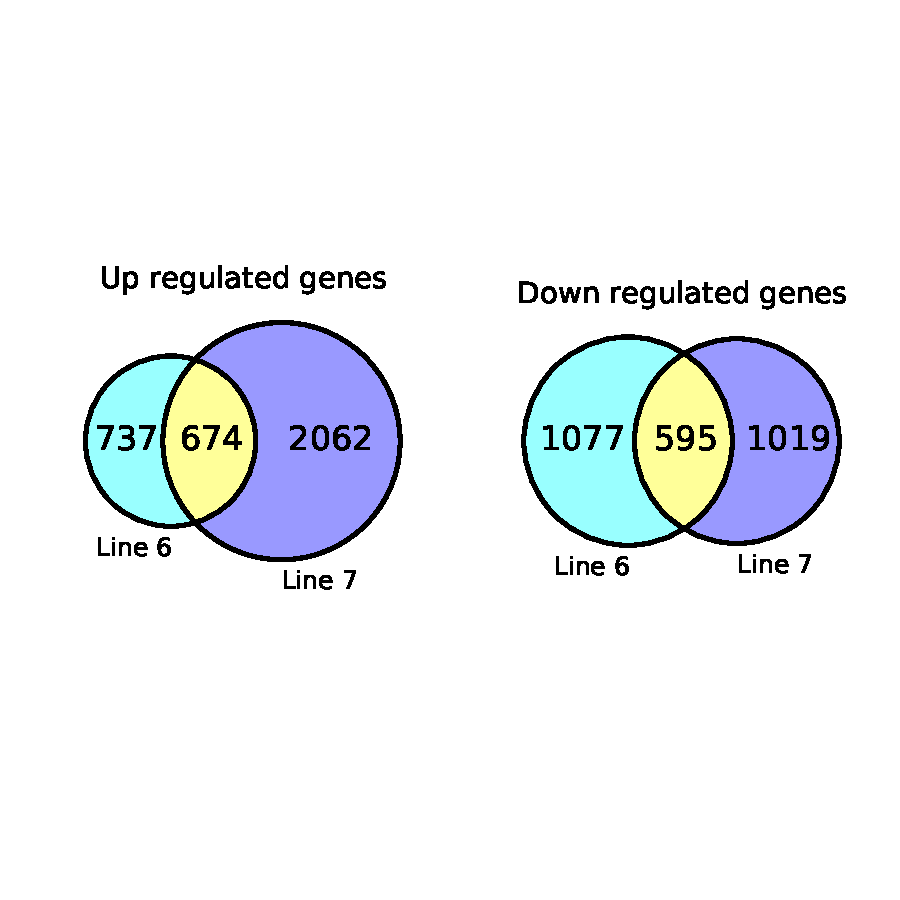
\includegraphics[width=6in]{degenes_venn.pdf}
    \end{center}
    \caption{
        {\bf Differential-expressed genes in response to MDV infection}
    }
    \label{degenes_venn}
\end{figure}

\begin{figure}[!ht]
    \begin{center}
        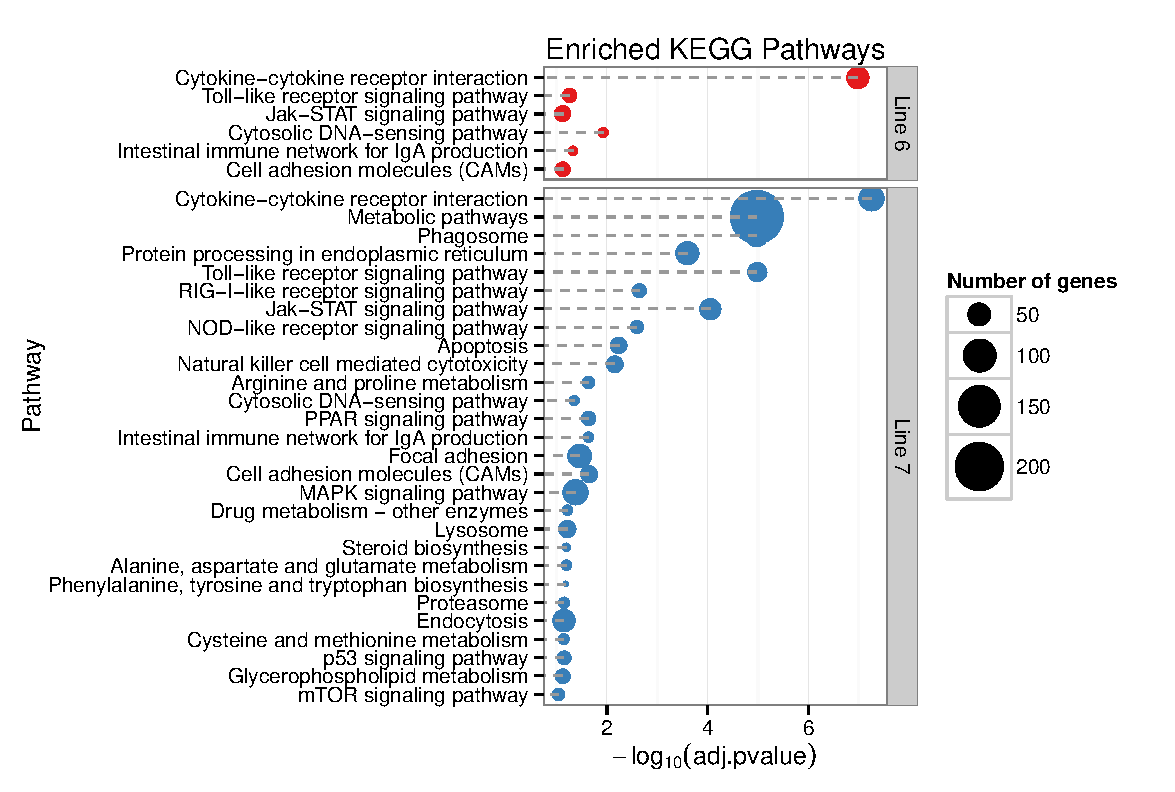
\includegraphics[width=7in]{line67_KEGG_cleveland.pdf}
    \end{center}
    \caption{
        {\bf Enriched KEGG pathways.}
    }
    \label{line67_kegg}
\end{figure}

\begin{figure}[!ht]
    \begin{center}
        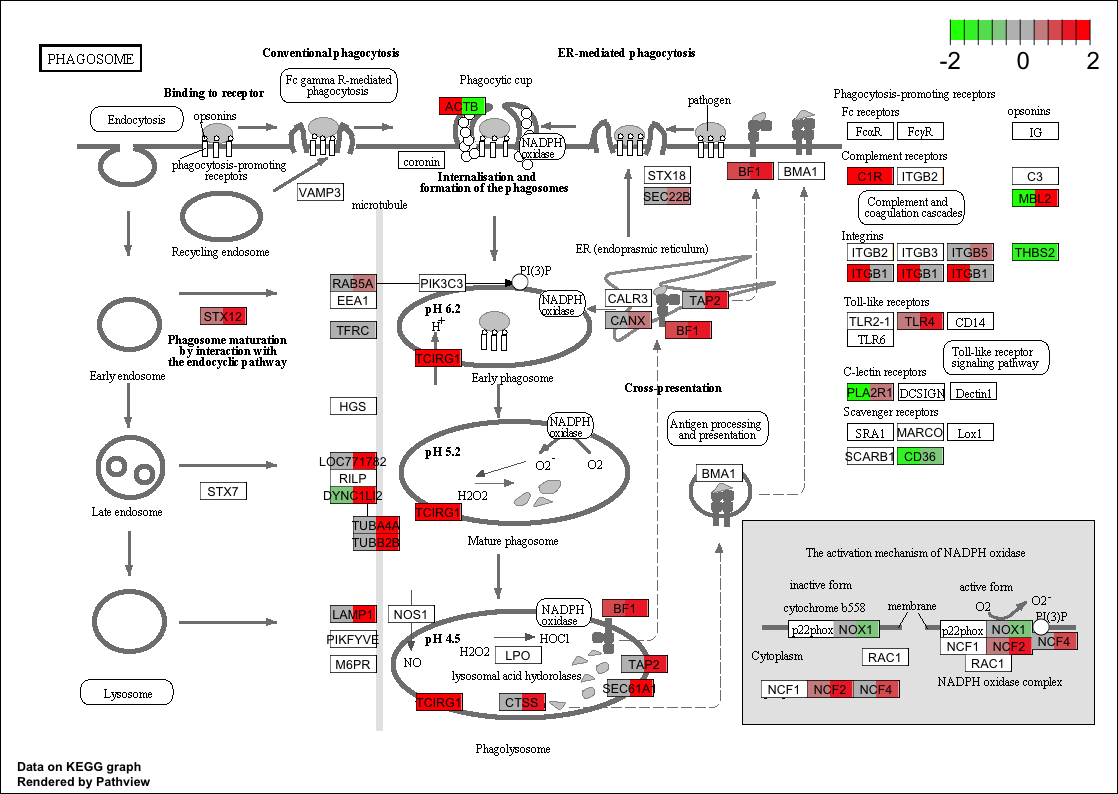
\includegraphics[width=6in]{gga04145_degenes_multi.png}
    \end{center}
    \caption{
        {\bf Phagosome pathway.}
    }
    \label{kegg_phagosome}
\end{figure}

\begin{figure}[!ht]
    \begin{center}
        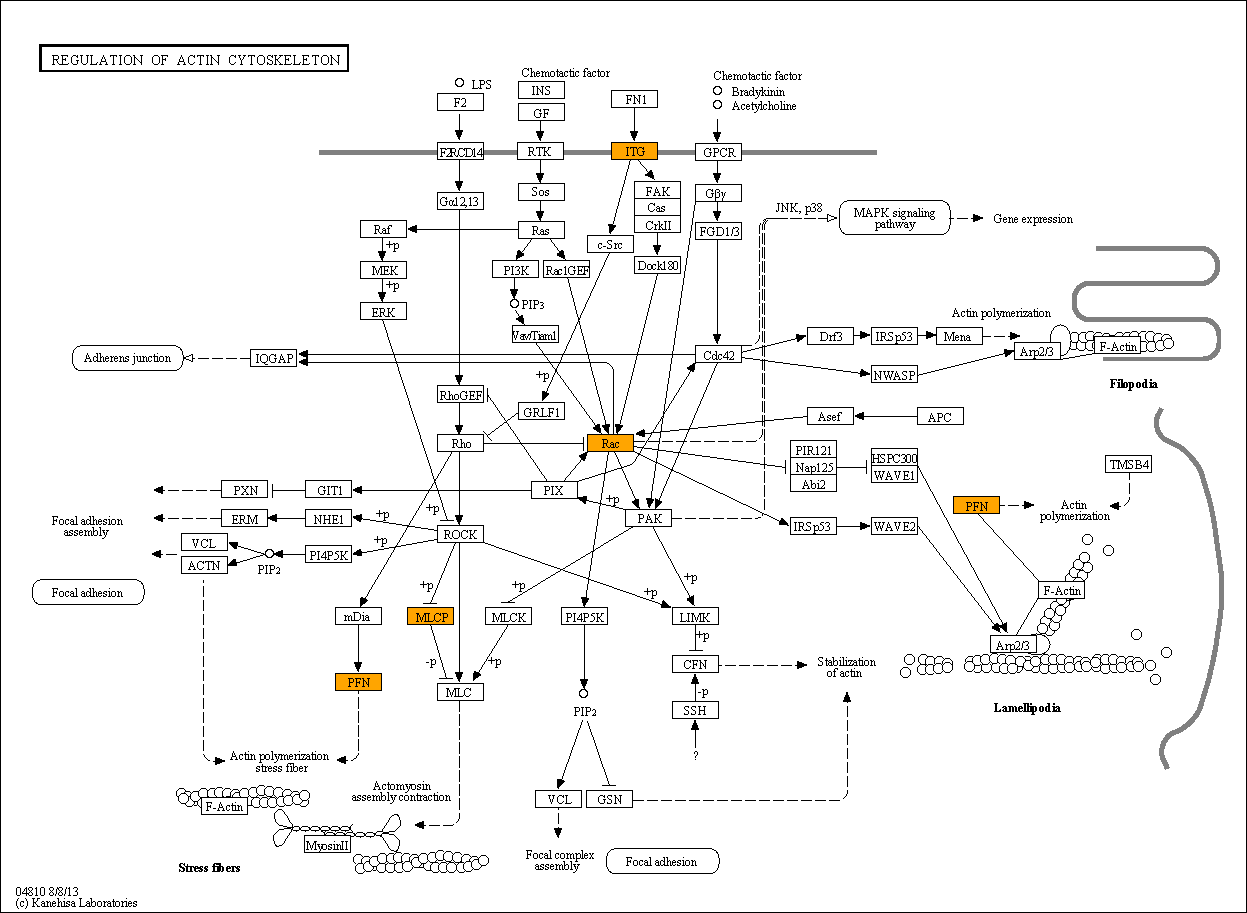
\includegraphics[width=6in]{hsa04810_deu_genes.png}
    \end{center}
    \caption{
        {\bf Human regulation of actin cytosekeleton pathway.}
    }
    \label{kegg_actin}
\end{figure}

\begin{figure}[!ht]
    \begin{center}
        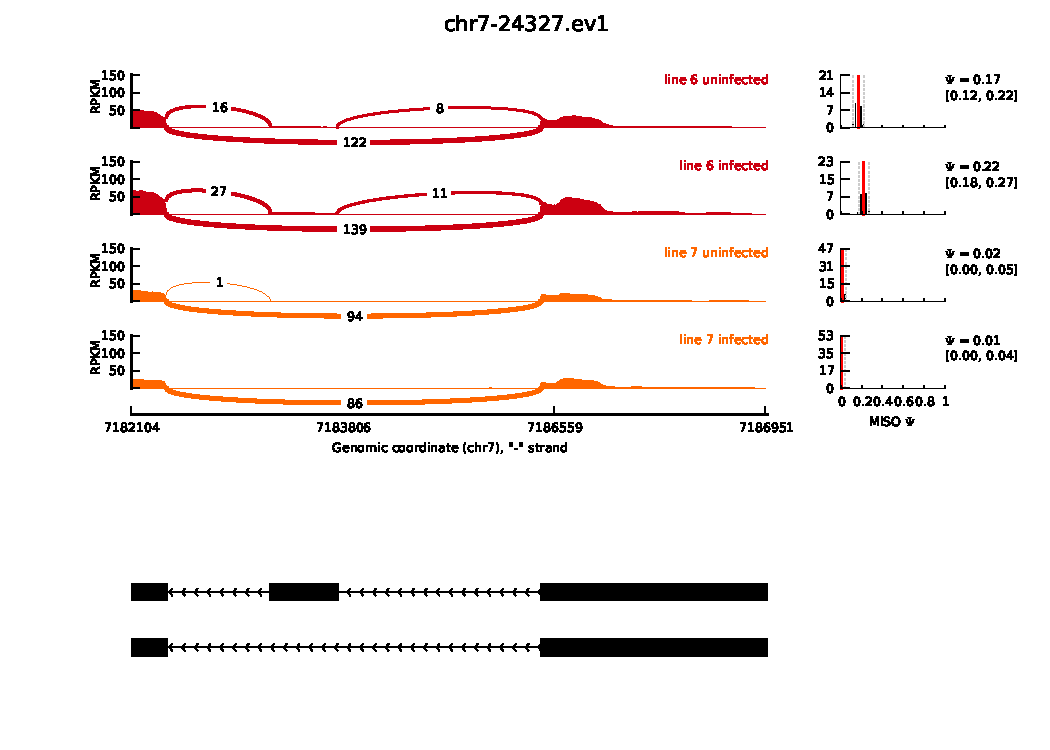
\includegraphics[width=6in]{itgb2_miso.pdf}
    \end{center}
    \caption{
        {\bf ITGB2 exon expression.}
        A single nuclotide substition (T$>$C) at position 7,183,696 is predicted to disrupt a putative ESE
        motif which binds SC35 on the skipped exon of IRGB2 gene shown in this figure.
        The prediction correlate with exclusion of the exon in line 7 ($\Psi \leq 0.02$).
        A new binding site for a silencer is also predicted and could also promote the exclusion of the exon. 
    }
    \label{itgb2}
\end{figure}

\begin{figure}[!ht]
    \begin{center}
        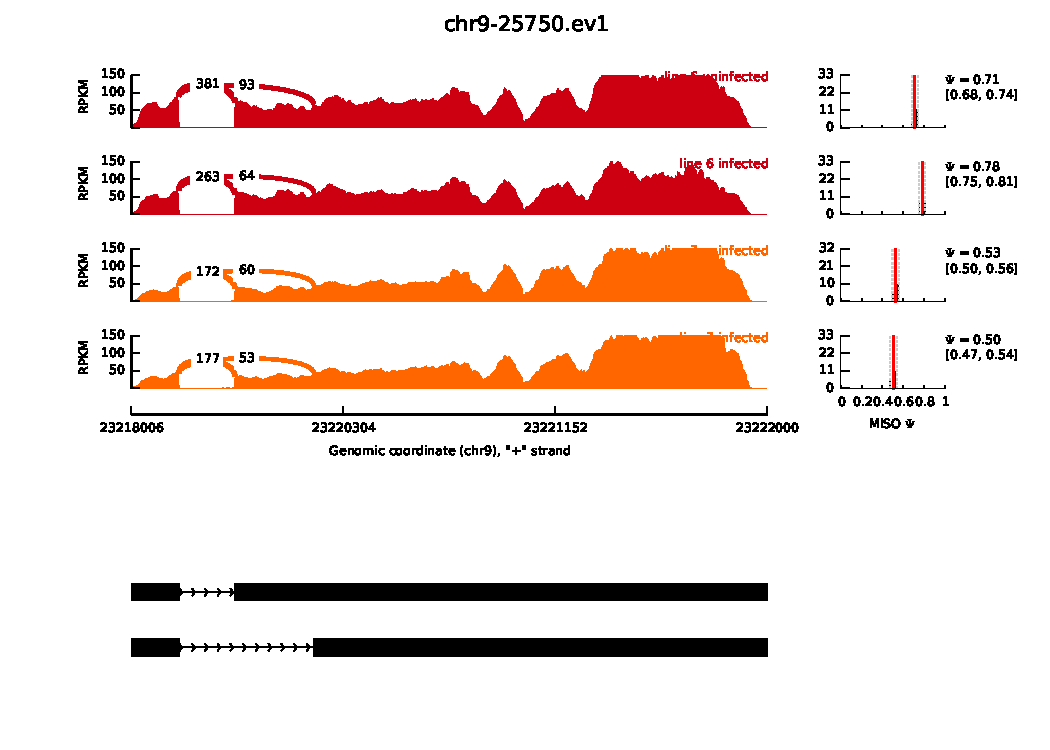
\includegraphics[width=6in]{pfn2_miso.pdf}
    \end{center}
    \caption{
        {\bf PFN2 exon expression.}
        A small insertion of AA nucleotides at position 23,221,934 is predicted to create a putative ESE motif
        which binds to Tra2 protein.
        Tra2 could promote inclusion of exon with alternative 3$\prime$ splice site via ESE-dependent
        3$\prime$ splice site activation resulting in higher expression of the exon in line 7.
        Even though the predicted ESE motif is located at a substantial distance from the alternative 3$\prime$ splice site,
        Tra2 could still regulate the splicing if a secondary structure of the mRNA moves the ESE motif closer to the
        alternative 3$\prime$ splice site.
    }
    \label{pfn2}
\end{figure}

\section*{Tables}

% \begin{table}[!ht]
%     \caption{
%     \bf{Gene models summary}}
%     \begin{tabular}{ccc}
%         \hline
%         Method & Gene & Isoform \\
%         \hline
%         Assembly & 25,290 & 54,044 \\
%         Cufflinks & 21,345 & 36,218 \\
%         Combined & 24,980 & 46,613 \\
%         \hline
%     \end{tabular}
%     \begin{flushleft}
%         Number of genes and isoforms from gene models
%         built from {\em de novo} assembly and Cufflinks.
%         Combination of both methods decreased the number of genes
%         and isoforms by merging fragmented transcripts to
%         form more complete gene models.
%     \end{flushleft}
%     \label{tab:gene_models}
% \end{table}

\begin{table}[!ht]
\caption{
\bf{Genes regulated in opposite directions}}
    \begin{tabular}{cccc}
        \hline
        Gene & Description & $log_{2}$FC & \\
         & & Line 6 & Line 7 \\
        \hline
        LL & Lung lectin & -3.36 & 8.70 \\
        GIF & Gastric intrinsic factor & -2.15 & 3.11 \\
        SFTPA1 & Surfactant protein A1 & -4.84 & 3.73 \\
        SCAF8 & SR-related CTD-associated factor 8 & -8.70 & 8.24 \\
        LIMS1 & LIM and senescent cell antigen-like domains 1 & -2.26 & 1.33 \\
        PPARG & Peroxisome proliferator-activated receptor gamma & -6.99 & 2.06 \\
        C14ORF1 & Chromosome 14 open reading frame 1 & -3.11 & 2.71 \\
        Unknown & Unknown & -3.08 & 1.62 \\
        \hline
        ATP8A2 & ATPase, aminophospholipid transporter, class I, type 8A, member 2 & 7.66 & -7.80 \\
        S1PR1 & Sphingosine-1-phosphate receptor 1 & 1.31 & -6.95 \\
        MED9 & Mediator complex subunit 9 & 8.22 & -3.15 \\
        DNAJA2 & DnaJ (Hsp40) homolog, subfamily A, member 1 & 2.34 & -6.02 \\
        RAD17 & RAD17 homolog (S. pombe) & 1.45 & -1.80 \\
        PSMG3 & Proteosome assembly chaperone 3 & 1.52 & -1.26 \\
        PNISR & PNN-interacting serine/argining-rich protein & 5.58 & -1.81 \\
        THOC7 & THO complex 7 homolog (Drosophila) & 7.00 & -6.90 \\
        YTHDC2 & YTH domain containing 2 & 1.00 & -1.74 \\
        RPL39 & Ribosomal protein L39 & 3.31 & -1.59 \\
        CD7 & CD7 molecule & 2.88 & -1.38 \\
        NDUFB3 & NADH dehydrogenase (uqiquinone) 1 beta subcomplex 3 & 1.03 & -1.34 \\
        LOC100858785 & Unknown & 1.26 & -1.75 \\
        Unknown & Unknown & 6.30 & -5.22 \\
        \hline
    \end{tabular}
    \begin{flushleft}
        (-) down-regulated, (+) up-regulated
    \end{flushleft}
    \label{tab:opposite}
\end{table}

\begin{table}[!ht]
\caption{
\bf{Cytokine-related gene expression in response to MDV infection}}
    \begin{tabular}{cccccc}
        \hline
        & & $log_{2}$FC & \\
        Symbol & Description & Line 6 & Line 7 \\
        \hline
        IL2RG & Interleukin 2 receptor, $\gamma$ & -- & 0.55 \\
        IL6 & Interleukin 6 (interferon, $\beta$ 2) & -- & 5.15 \\
        IL6ST & Interleukin 6 signal transducer (gp130, oncostatin M receptor) & -- & 1.36 \\
        IL8L1 & Interleukin 8-like 1 & 1.90 & -- \\
        IL15 & Interleukin 15 & -- & 1.06 \\
        IL18 & Interleukin 18 (interferon-$\gamma$ inducing factor) & 1.92 & 4.06 \\
        IL18R1 & Interleukin 18 receptor 1 & 1.94 & 1.64 \\
        IFNG & Interferon-$\gamma$ & 5.14 & 4.90 \\
        IFNB & Interferon-$\beta$ & 4.83 & 5.64 \\
        IFNA3 & Interferon-$\alpha$ 3 & 4.09 & 5.48 \\
        IFNGR1 & Interferon-$\gamma$ receptor 1 & -- & 2.05 \\
        IFNGR2 & Interferon-$\gamma$ receptor 2& -- & 0.50 \\
        IFNAR1 & Interferon-$\alpha$,$\beta$ receptor 1 & -- & 1.46 \\
        IFNAR2 & Interferon-$\alpha$,$\beta$ receptor 2 & -- & 0.58 \\
        \hline
    \end{tabular}
    \begin{flushleft}
    \end{flushleft}
    \label{tab:cytokines}
\end{table}

\begin{table}[!ht]
\caption{
\bf{DEU between Line 6 and Line 7 in infected birds group I}}
\begin{tabular}{cccccccc}
\hline
& & & & Line 6 ($\Psi$) & & Line 7 ($\Psi$) & \\
Type & Event ID & Ensembl & Symbol  & Un & Inf & Un & Inf \\
\hline
SE & chr2:13729.ev2 & ENSGALG00000010973 & \textbf{TRA2A} & 0.45 & \textbf{0.75} & 0.58 & 0.50 \\
SE & chr5:22858.ev1 & ENSGALG00000011127 & BCL11B & 0.07 & \textbf{0.30} & 0.06 & 0.04 \\
SE & chr2:13065.ev1 & ENSGALG00000013137 & INO80C & 0.14 & \textbf{0.35} & 0.96 & 0.86 \\
SE & chr20:14995.ev1 & ENSG00000124193* & SRSF6 & 0.43 & \textbf{0.72} & 0.54 & 0.34 \\
A5SS & chr7:24049.ev1 & ENSGALG00000009824 & \textbf{C7H2ORF77} & 0.50 & \textbf{0.73} & 0.32 & 0.38 \\
A5SS & chr3:18098.ev1 & ENSGALG00000013821 & \textbf{GEMIN6} & 0.84 & \textbf{0.61} & 0.81 & 0.85 \\
A3SS & chr1:6450.ev1 & ENSGALG00000027665 & \textbf{SYNGR1} & 0.46 & \textbf{0.22} & 0.68 & 0.60 \\
A3SS & chr2:13270.ev1 & ENSGALG00000026498 & \textbf{Unknown} & 0.12 & \textbf{0.71} & 0.10 & 0.34 \\
A3SS & chr19:12399.ev1 & ENSGALG00000005685 & \textbf{KSR1} & 0.23 & \textbf{0.56} & 0.28 & 0.35 \\
A3SS & chr1:6437.ev1 & ENSGALG00000012050 & \textbf{TNRC6B} & 0.57 & \textbf{0.39} & 0.95 & 0.93 \\
A3SS & chr18:11800.ev1 & ENSGALG00000002859 & \textbf{RAC3} & 0.31 & \textbf{0.15} & 0.33 & 0.39 \\
\hline
\end{tabular}
\begin{flushleft}
    *human homologs, Un=uninfected, Inf=infected.
    Bold face indicates that there is a SNP between line 6 and 7 within an alternative exon.
\end{flushleft}
\label{tab:line67i_diff_line67u_one}
\end{table}

\begin{table}[!ht]
\caption{
\bf{DEU between Line 6 and Line 7 in infected birds group II}}
\begin{tabular}{cccccccc}
\hline
& & & & Line 6 ($\Psi$) & & Line 7 ($\Psi$) & \\
Type & Event ID & Ensembl & Symbol  & Un & Inf & Un & Inf \\
\hline
SE & chr17:11370.ev2 & ENSGALG00000004971 & URM1 & \textbf{0.07} & \textbf{0.03} & 0.18 & 0.23 \\
SE & chr2:12495.ev3 & ENSGALG00000005582 & \textbf{KLHL18} & \textbf{0.44} & \textbf{0.27} & 0.56 & 0.52 \\
SE & chr7:24327.ev1 & ENSGALG00000007511 & \textbf{ITGB2} & \textbf{0.17} & \textbf{0.22} & 0.02 & 0.01 \\
SE & chr2:12984.ev1 & ENSGALG00000012809 & ECI2 & \textbf{0.15} & \textbf{0.29} & 0.58 & 0.49 \\
SE & chr8:25247.ev1 & ENSGALG00000028790 & DNASE2B & \textbf{0.38} & \textbf{0.50} & 0.29 & 0.26 \\
SE & chr1:4653.ev1 & ENSGALG00000011682 & CNOT4 & \textbf{0.57} & \textbf{0.63} & 0.40 & 0.40 \\
SE & chr20:14907.ev3 & ENSGALG00000006522 & \textbf{HCK} & \textbf{0.46} & \textbf{0.59} & 0.99 & 0.97 \\
SE & chr4:21539.ev1 & ENSGALG00000015709 & \textbf{TACC3} & \textbf{0.87} & \textbf{0.94} & 0.76 & 0.72 \\
SE & chr2:32201.ev1 & ENSGALG00000012258 & GOLGA4 & \textbf{0.33} & \textbf{0.34} & 0.51 & 0.61 \\
SE & chr3:19470.ev1 & ENSGALG00000019979 & DYNLT1 & \textbf{0.23} & \textbf{0.22} & 0.02 & 0.02 \\
SE & chr19:12391.ev1 & ENSGALG00000005522 & \textbf{DYNLL2} & \textbf{0.01} & \textbf{0.02} & 0.19 & 0.25 \\
A5SS & chr6:23812.ev1 & ENSG00000107651* & \textbf{SEC23IP} & \textbf{0.02} & \textbf{0.12} & 0.50 & 0.43 \\
A5SS & chr2:12775.ev1 & ENSGALG00000011488 & \textbf{CMTM7} & \textbf{0.55} & \textbf{0.67} & 0.37 & 0.41 \\
A3SS & chr8:25257.ev1 & ENSGALG00000008939 & FUBP1 & \textbf{0.58} & \textbf{0.74} & 0.41 & 0.46 \\
A3SS & chr9:25750.ev1 & ENSGALG00000010410 & \textbf{PFN2} & \textbf{0.71} & \textbf{0.78} & 0.53 & 0.50 \\
A3SS & chr4:21230.ev1 & ENSGALG00000011476 & \textbf{SEPT11} & \textbf{0.22} & \textbf{0.14} & 0.40 & 0.42 \\
A3SS & chr4:20185.ev1 & ENSGALG00000008507 & THOC2 & \textbf{0.48} & \textbf{0.47} & 0.31 & 0.22 \\
A3SS & chr11:8703.ev1 & ENSGALG00000020987 & \textbf{ZDHHC7} & \textbf{0.42} & \textbf{0.23} & 0.57 & 0.55 \\
A3SS & chr4:21136.ev1 & ENSGALG00000027908 & \textbf{LOC422528} & \textbf{0.72} & \textbf{0.61} & 0.87 & 0.91 \\
\hline
\end{tabular}
\begin{flushleft}
    *human homologs, Un=uninfected, Inf=infected.
    Bold face indicates that there is a SNP between line 6 and 7 within an alternative exon.
\end{flushleft}
\label{tab:line67i_diff_line67u_two}
\end{table}

\begin{table}[!ht]
\caption{
\bf{DEU between Line 6 and Line 7 in infected birds group III and IV}}
\begin{tabular}{cccccccc}
\hline
& & & & Line 6 ($\Psi$) & & Line 7 ($\Psi$) & \\
Type & Event ID & Ensembl & Symbol  & Un & Inf & Un & Inf \\
\hline
SE & chr12:8987.ev1 & ENSGALG00000008320 & EDEM1 & 0.96 & 0.99 & 0.91 & \textbf{0.72} \\
SE & chr4:20411.ev1 & ENSGALG00000023199 & HNRPDL & 0.39 & 0.40 & 0.30 & \textbf{0.18} \\
SE & chrZ:26257.ev1 & ENSGALG00000001745 & PSTPIP2 & 0.06 & 0.04 & 0.13 & \textbf{0.26} \\
SE & chr1:6316.ev3 & ENSG00000058272* & PPP1R12A & 0.99 & 0.97 & 0.96 & \textbf{0.77} \\
SE & chr1:4478.ev2 & ENSGALG00000009029 & TSPAN12 & 0.09 & 0.15 & 0.20 & \textbf{0.46} \\
SE & chr4:20075.ev1 & ENSGALG00000006157 & DDX26B & 0.67 & 0.61 & 0.58 & \textbf{0.84} \\
SE & chr6:23515.ev1 & ENSGALG00000003861 & HERC4 & 0.31 & 0.37 & 0.45 & \textbf{0.06} \\
SE & chr26:16840.ev1 & ENSGALG00000000533 & SRSF3 & 0.36 & 0.38 & 0.30 & \textbf{0.16} \\
SE & chr11:8507.ev2 & ENSGALG00000000904 & \textbf{C11H16ORF57} & 0.91 & 0.98 & 0.84 & \textbf{0.78} \\
SE & chr1:4323.ev1 & ENSGALG00000006409 & PODXL & 0.21 & 0.34 & 0.26 & \textbf{0.13} \\
SE & chrZ:26582.ev2 & ENSGALG00000014642 & LOC374195 & 0.60 & 0.57 & 0.70 & \textbf{0.81} \\
SE & chr6:23833.ev1 & ENSG00000175029* & CTBP2 & 0.38 & 0.38 & 0.23 & \textbf{0.12} \\
A5SS & chr15:10720.ev1 & ENSGALG00000002487 & \textbf{SFSWAP} & 0.58 & 0.73 & 0.55 & \textbf{0.41} \\
A5SS & chr7:24350.ev1 & ENSGALG00000008038 & \textbf{SF3B1} & 0.41 & 0.57 & 0.55 & \textbf{0.31} \\
A3SS & chr2:13147.ev1 & ENSGALG00000014915 & \textbf{THOC1} & 0.33 & 0.48 & 0.33 & \textbf{0.23} \\
A3SS & chr23:15908.ev1 & ENSGALG00000000720 & LOC419563 & 0.12 & 0.06 & 0.17 & \textbf{0.30} \\
A3SS & chr8:25157.ev1 & ENSGALG00000005162 & RNPC3 & 0.45 & 0.64 & 0.58 & \textbf{0.33} \\
A3SS & chrZ:27197.ev1 & ENSGALG00000000189 & \textbf{YTHDC2} & 0.44 & 0.59 & 0.42 & \textbf{0.32} \\
A3SS & chr23:15983.ev1 & ENSG00000163875* & \textbf{MEAF6} & 0.28 & 0.57 & 0.40 & \textbf{0.29} \\
A3SS & chr5:21970.ev1 & ENSGALG00000009421 & \textbf{SRSF5} & 0.55 & 0.72 & 0.54 & \textbf{0.39} \\
\hline
SE & chr27:17351.ev1 & ENSGALG00000001107 & GOSR2 & 0.73 & 0.92 & 0.38 & 0.60 \\
\hline
\end{tabular}
\begin{flushleft}
    *human homologs, Un=uninfected, Inf=infected.
    Bold face indicates that there is a SNP between line 6 and 7 within an alternative exon.
\end{flushleft}
\label{tab:line67i_diff_line67u_three}
\end{table}

\begin{table}[!ht]
\caption{
\bf{Pathways containing {\em RAC3, ITGB2, PFN2} and {\em PPP1R12A}}}
\begin{tabular}{ccc}
\hline
Pathway ID &  Description & Gene \\
\hline
hsa04810 & Regulation of actin cytoskeleton & {\em RAC3, ITGB2, PPP1R12A, PFN2} \\
hsa04015 & RAP1 signaling pathway & {\em RAC3, ITGB2, PFN2} \\
hsa04650 & Natural killer cells cytotoxicity & {\em RAC3, ITGB2} \\
hsa05416 & Viral myocarditis & {\em RAC3, ITGB2} \\
hsa04510 & Focal adhesion & {\em RAC3, PPP1R12A} \\
\hline
\end{tabular}
\begin{flushleft}
\end{flushleft}
\label{tab:integrin}
\end{table}

\begin{table}[!ht]
\caption{
\bf{SNPs in exons}}
\begin{tabular}{ccccccc}
\hline
Gene &  Chromosome & Position & Reference & Line 6 & Line 7 & Strand \\
\hline
ITGB2 & 7 & 7183696 & C & {\em T} & . & - \\
PFN2 & 9 & 23221934 & -  - & . & {\em AA} & + \\
DYNLT1 & 3 & 51357865 & C & . & {\em G} & - \\
DYNLL2 & 19 & 8694148 & G & . & {\em A} & - \\
\hline
\end{tabular}
\begin{flushleft}
\end{flushleft}
\label{tab:deu_snps}
\end{table}

\begin{table}[!ht]
\caption{
\bf{Results from human splicing finder}}
\begin{tabular}{|l|p{1cm}|p{3cm}|l|l|l|l|}
\hline
Gene &  cDNA Position & Linked SR protein & Type & Reference Motif & Mutant Motif & Variation \\
\hline
% ITGB2 & 20 & SC35 & ESE$^{1}$ & TGCTCATG (78.19) & & Site broken \\
%  & 22 & SF2/ASF(IgM-BRCA1) & ESE$^{1}$ & CTCATGG (77.23) & CTCACGG (91.15) & +18.03\% \\
%  & 22 & SF2/ASF(IgM-BRCA1), SF2/ASF & ESE$^{1}$ & CTCATGG (77.23) & CTCACGG (89.23) & +15.53\% \\
%  & 22 & SF2/ASF, SF2/ASF(IgM-BRCA1) & ESE$^{1}$ & CTCATGG (74.55) & CTCACGG (91.15) & +22.27\% \\
%  & 22 & SF2/ASF, SF2/ASF & ESE$^{1}$ & CTCATGG (74.55) & CTCACGG (89.23) & +19.69\% \\
%  & 24 & SRp55 & ESE$^{1}$ & & CACGGA (79.30) & New site \\
%  & 26 & SF2/ASF(IgM-BRCA1) & ESE$^{1}$ & & CGGAGAT (80.00) & New site \\
%  & 26 & SF2/ASF & ESE$^{1}$ & & CGGAGAT (75.36) & New site \\
%  & 21 & & ESS$^{3}$ & & GCTCACGG (63.35) & New site (-5.59) \\
%  & 23 & & ESS$^{3}$ & TCATGGAG (61.41) & & Site broken (3.16) \\
%  & 23 & & ESS$^{3}$ & ATGGAGAT (64.83) & ACGGAGAT & -5.16\% \\
%  & 24 & & ESS$^{4}$ & CATGGA (65.48) & CACGGA (65.48) & 0\% \\
DYNLT1 & 59 & SRp55, SRp40 & ESE$^{1}$& TGAATC (78.47) & TGAATGC (79.10) & +0.81\% \\
& 60 & 9G8 & ESE$^{2}$ & GAATCC (60.07) & GAATGC (63.49) & +5.70\% \\
\hline
DYNLL2 & 2 & SF2/ASF (IgM-BRCA1) & ESE$^{1}$ & CTCCGGG (86.38) & CTCCGAG (72.69) & -15.85\% \\
& 2 & SF2/ASF, SF2/ASF (IgM-BRCA1) & ESE$^{1}$ & CTCCGGG (79.91) & CTCCGAG (72.69) & -9.03\% \\
& 4 & SF2/ASF (IgM-BRCA1) & ESE$^{1}$& CCGGGGT (73.00) & CCGAGGT (86.23) & 18.12\% \\
& 4 & SF2/ASF (IgM-BRCA1), SF2/ASF & ESE$^{1}$ & CCGGGGT (73.00) & CCGAGGT (82.94) & 13.61\% \\
& 6 & 9G8 & ESE$^{2}$ & & GAGGTG (60.67) & New site \\
& 6 & hnRNP A1 & ESS$^{4}$& & GAGGTG (74.05) & New site \\
\hline
PFN2 & 2068 & Tra2-$\beta$ & ESE$^{1}$ & AAAAT (81.02) & AAAAa & +16.19\% \\
& 2069 & Tra2-$\beta$ & ESE$^{1}$ & & AAAaa (94.14) & New site \\
& 2070 & Tra2-$\beta$ & ESE$^{1}$ & & AAAaaT (81.02) & New site \\
 & 2066 & & ESS$^{3}$ & & ACAAAAaa (38.13) & New site \\
 & 2067 & & ESS$^{3}$ & & CAAAAaaT (28.85) & New site \\
\hline

\end{tabular}
\begin{flushleft}
    $^{1}$ESE Finder matrices for SRp40, SC35, SF2/ASF and SRp55 proteins.
    $^{2}$ESE motifs from HSF.
    $^{3}$Predicted PESS Octamers from Zhang \& Chasin.
    $^{4}$hnRNP motif.
\end{flushleft}
\label{tab:spliceosome}
\end{table}

\end{document}
